\documentclass{beamer}

% For more themes, color themes and font themes, see:
% http://deic.uab.es/~iblanes/beamer_gallery/index_by_theme.html
%
\mode<presentation>
{
  \usetheme{Madrid}       % or try default, Darmstadt, Warsaw, ...
  \usecolortheme{default} % or try albatross, beaver, crane, ...
  \usefonttheme{serif}    % or try default, structurebold, ...
  \setbeamertemplate{navigation symbols}{}
  \setbeamertemplate{caption}[numbered]
} 

\usepackage{tikz}
\usetikzlibrary{decorations.markings,angles}
\usepackage{tikz-3dplot} 

\usepackage{amsmath}


\begin{document}


\begin{frame}{CanariCam}

\begin{itemize}
\item CanariCam is a mid-infrared imager with spectroscopic, coronagraphic, and polarimetric capabilities. \\~\\

\item It is optimized for excellent image quality across the 8-26 $\mu m$  window. The optical design is such that CanariCam is diffraction limited at 8 $\mu m$ (Nyquist sampling the 8 μm PSF).
\end{itemize}
\end{frame}


\begin{frame}{Gran telescopio de canarias (GTC)}
\begin{columns}
\begin{column}{0.45\textwidth}
\begin{center}
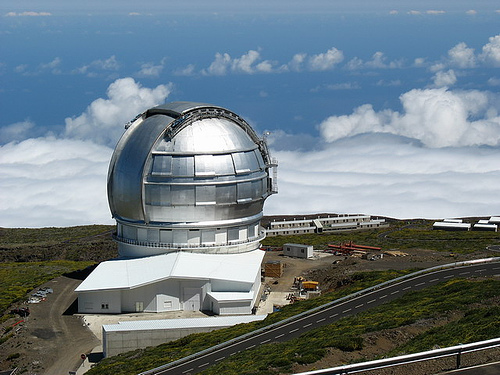
\includegraphics[scale=0.30]{imgr2.png}
\end{center}
\end{column}

\begin{column}{0.45\textwidth}
\begin{center}
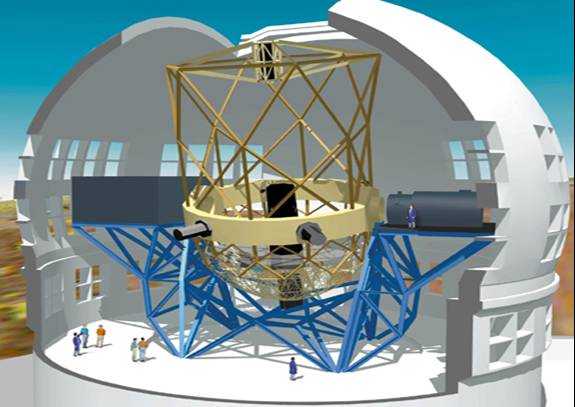
\includegraphics[height=0.41\textheight]{imgr1.png}
\end{center}
\end{column}
\end{columns}
\end{frame}




\begin{frame}{Optical layout}

\begin{itemize}
\item There are three powered mirrors and five folding flats (four fixed and one movable on the grating turret). All the mirrors are gold coated, which provides a combined reflectivity of $92\%$. \\~\\

\item CanariCam is equipped with a suite of narrow-band and broad-band $10$ and $20~\mu m$ filters,
located within two filter wheels immediately after the Lyot-stop wheel at the first pupil
image.
\end{itemize}
\end{frame}

\begin{frame}{Optical Layout}

\begin{columns}

\begin{column}{0.5\textwidth}
\begin{center}
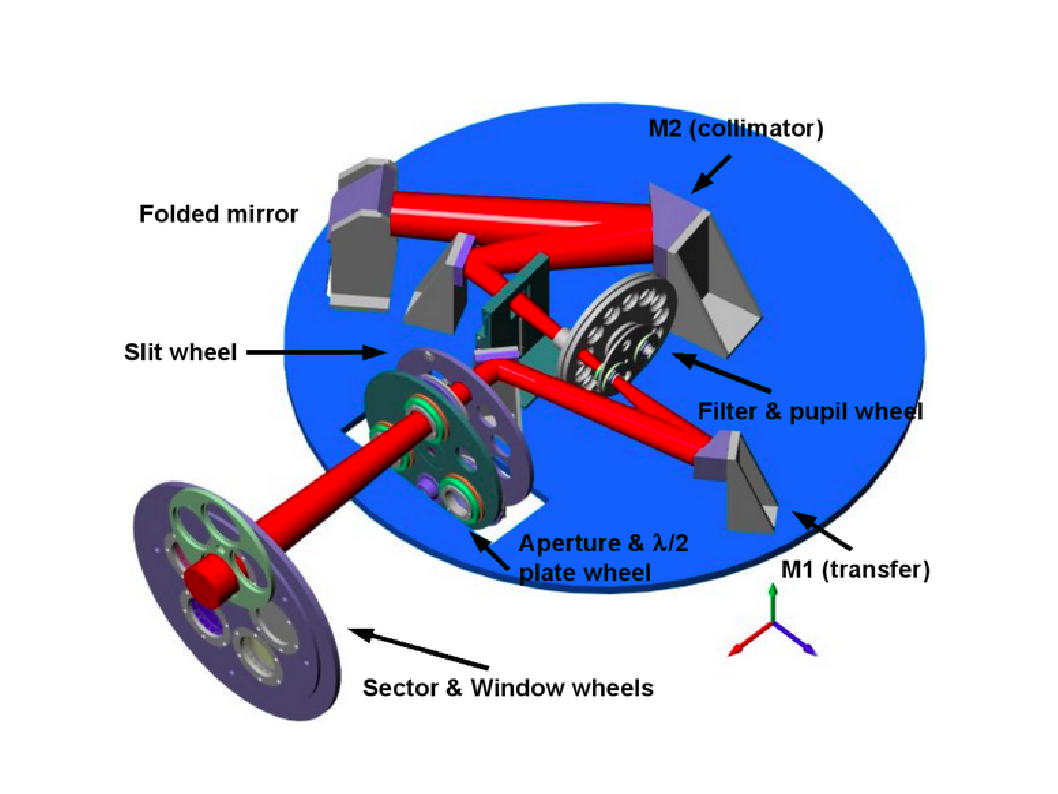
\includegraphics[scale=0.22]{imgr5.png}
\end{center}
\end{column}

\begin{column}{0.45\textwidth}
\begin{center}
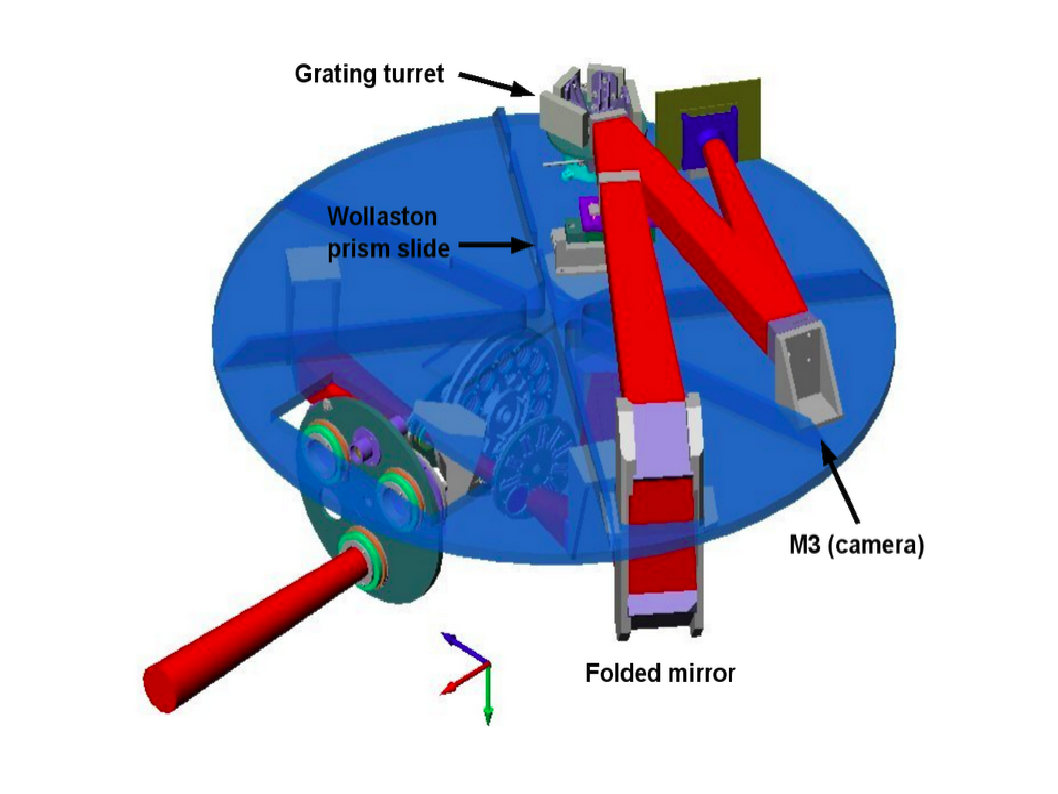
\includegraphics[scale=0.22]{imgr6.png}
\end{center}
\end{column}
\end{columns}
\end{frame}


\begin{frame}{Detector characteristics}
\begin{center}
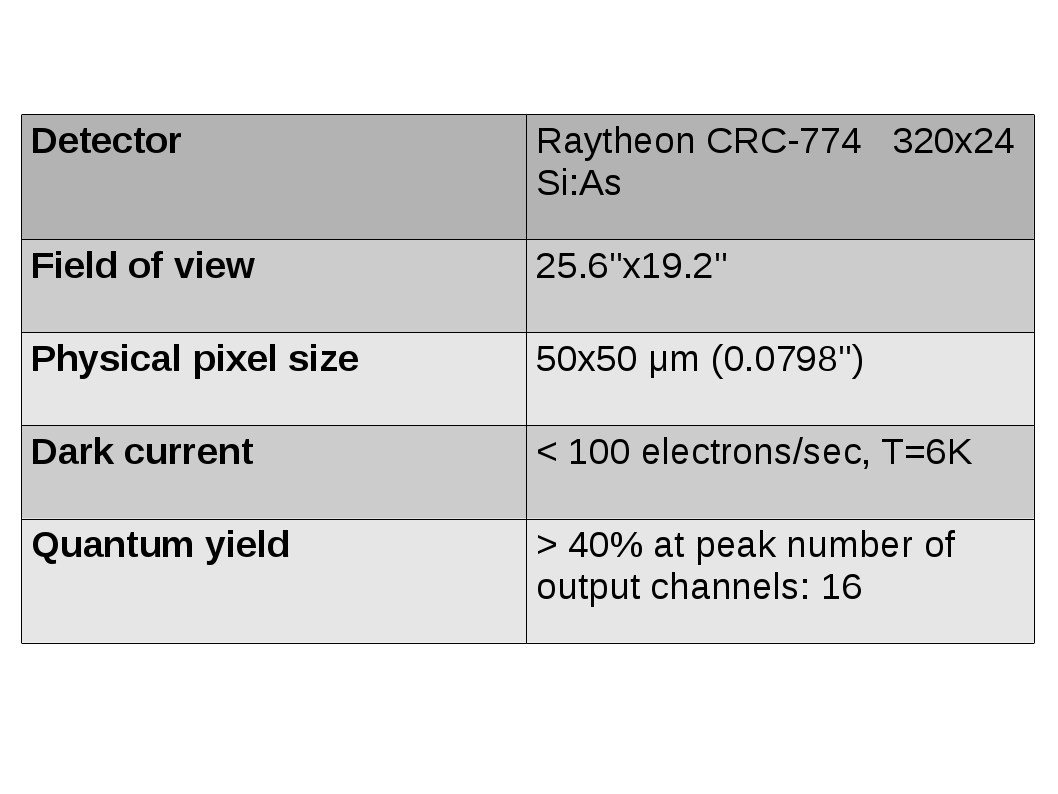
\includegraphics[scale=0.35]{imgr7.png}
\end{center}
\end{frame}

\begin{frame}{Quantum efficiency of detector}
\begin{center}
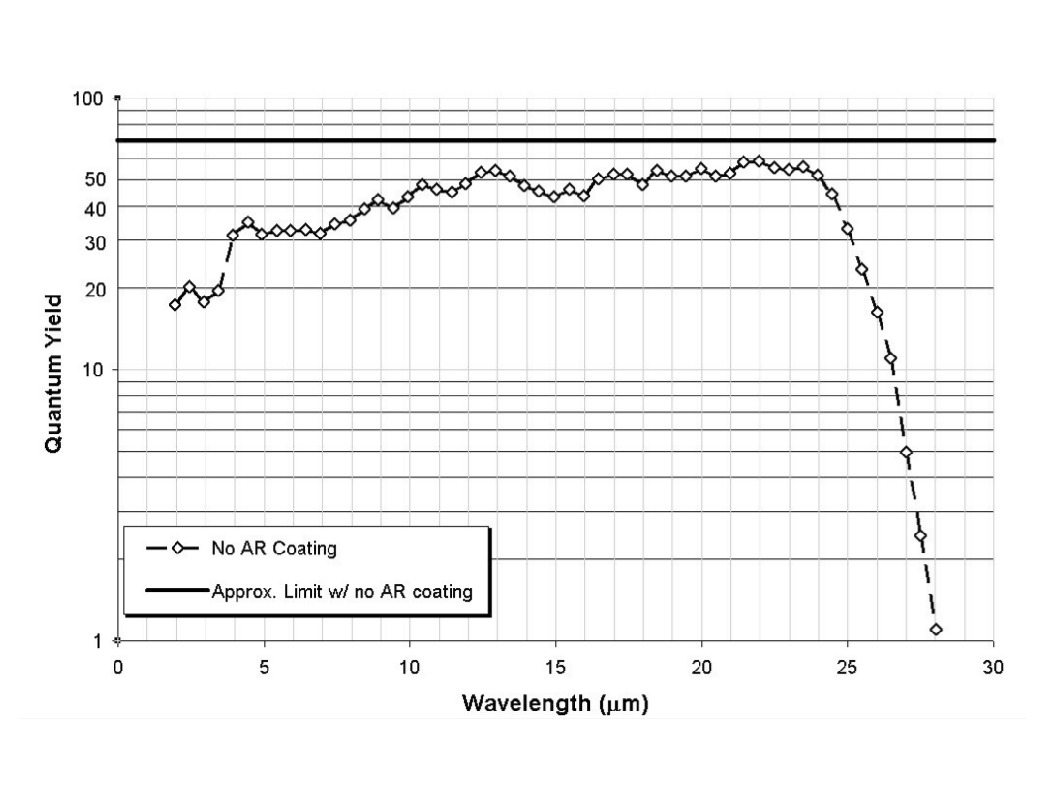
\includegraphics[scale=0.35]{imgr8.png}
\end{center}
\end{frame}


\begin{frame}{Spectroscopy}

R (spectral resolution) = $\frac{\lambda}{\delta \lambda}$  
is an adimensional measure of  $\delta \lambda$ (spectral purity or spectral resolution element):
the smallest measurable wavelength difference at a given wavelength

$R \propto \frac{\lambda A}{min(w,l_0)}$ and $A=\frac{d\beta}{d \lambda}$ is a decreasing function of $\lambda$

\begin{figure}[H]
 \centering
 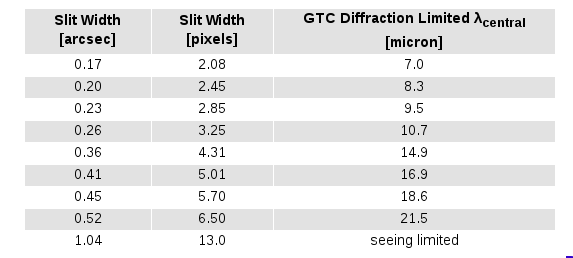
\includegraphics[scale=0.32]{img9.png}
\end{figure}
Typically for each grating there will be 2 slits available corresponding to the resolution and two times the resolution at the 
maximum wavelength (1 and 2 $\lambda$/D)
\end{frame}

\begin{frame}{Spectroscopy}
\begin{figure}[H]
 \centering
 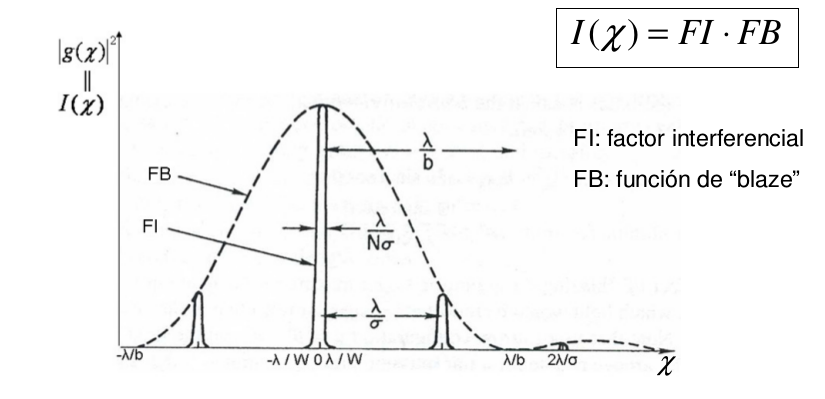
\includegraphics[scale=0.25]{img7.png}
\end{figure}
\begin{figure}[H]
 \centering
 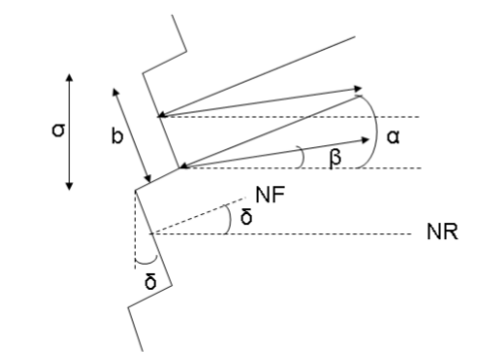
\includegraphics[scale=0.32]{img8.png}
\end{figure}

\end{frame}

\begin{frame}{Spectroscopy}
\begin{itemize}
\item $W = \sigma N$, $b = \sigma cos \delta$, $\chi = sin \alpha + sin \beta$
\item FI max when  $\frac{m \lambda}{\sigma} = sin \alpha + sin \beta$
\item FB max when $\alpha + \beta = 2 \delta$
\item $\alpha, \delta$ fixed $\implies $ max intensity when 
$\beta = 2 \delta - \alpha \implies \lambda_{max} = \frac{\sigma}{m}(sin \alpha + sin(2\delta - \alpha))$ 
which for m = 1 is called $\lambda_{blaze}$
\end{itemize}


\end{frame}

\begin{frame}{Spectroscopy}

10 $\mu $ window(7.5 - 13.5 $\mu m$ also called N band) low and high resolution grating
\begin{tabular}{|c|c|c|}
\hline
Characteristics & 	LR	& HR \\
\hline
Central $\lambda_c(\mu m)$	& 10.5	& 10.5 \\
\hline
Blaze $\lambda (\mu m)$ &	9.87	& 10.08 \\
\hline
Blaze Angle ($^{\circ}$) & 	2.6	& 16.4 \\
\hline
Lines/mm(N)	& 9.1 &	56.0 \\
\hline
$\delta \lambda_{Det} (\mu m)$ &	6	& 0.98 (0.65 for $\lambda_c = 10.5 \mu m$)\\
\hline
Angle of incidence ($^{\circ}$)	& 14.8 &	29.5\\
\hline
Angle diffraction ($^{\circ}$) at $\lambda_c$	& 9.2	& 5.5\\
\hline
R	& 175	& 1300\\
\hline
Smallest Resolvable $ \delta \lambda (\mu m)$ &	0.06	&0.008 \\
\hline
\end{tabular}
\end{frame}
\begin{frame}{Spectroscopy}

20 $\mu $ window (16.0 - 25.0 $\mu m$)  low and high resolution grating
\begin{tabular}{|c|c|c|}
\hline
Characteristics & 	LR	& HR \\
\hline
Central $\lambda_c(\mu m)$	& 20.5	& 20.5 \\
\hline
Blaze $\lambda (\mu m)$ &	19.96	& 20.18 \\
\hline
Blaze Angle ($^{\circ}$) & 	4.0	& 20.8 \\
\hline
Lines/mm(N)	& 6.1 &	35.2 \\
\hline
$\delta \lambda_{Det} (\mu m)$ &	9	& 1.54 ($0.45 \mu m$ for $\lambda_c = 20.5 \mu m$)\\
\hline
Angle of incidence ($^{\circ}$)	& 15.7 &	33.7\\
\hline
Angle diffraction ($^{\circ}$) at $\lambda_c$	& 8.3	& 9.7\\
\hline
R	& 120	& 890\\
\hline
Smallest Resolvable $ \delta \lambda (\mu m)$ &	0.17	&0.025 \\
\hline
\end{tabular}



\end{frame}

\begin{frame}{Spectroscopy}
Spectrum dispersed along the long axis of the array (320 pixels)

Each resolution element is sampled by approx. 5 pixels for low resolution gratings
\end{frame}

\begin{frame}{Spectroscopy(sensitivity)}
\begin{figure}[H]
 \centering
 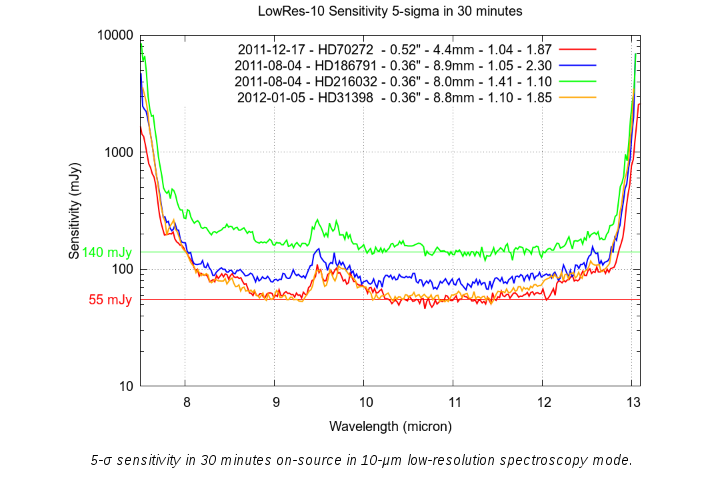
\includegraphics[scale=0.2]{img10.png}
\end{figure}
\begin{figure}[H]
 \centering
 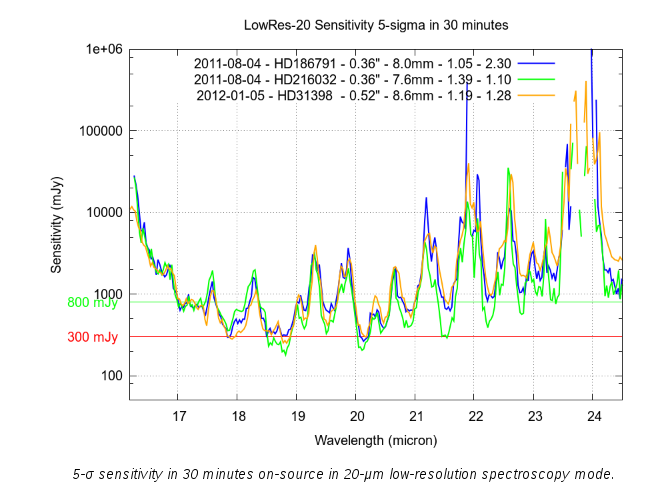
\includegraphics[scale=0.2]{img11.png}
\end{figure}

\end{frame}

\begin{frame}{Spectroscopy(sensitivity)}
At bluer wavelengths, where the PSF is narrower, there is a higher contribution from the background 
within the aperture than at redder wavelengths

In the case of 20 $\mu m$ window  there is a stronger dependency of the sensitivity with wavelength than in the 10 $\mu m$  window, 
due to the presence of strong water lines in the 20 $\mu m$ atmospheric window.
\end{frame}


\begin{frame}{Polarimetry}

\begin{itemize}
\item half wave plate (retarder with $\delta = \pi$)
\item  a focal plane mask which prevents overlap of the orthogonally polarized images for extended sources
\item cadmium selenide (CdSe) Wollaston prism (an optical device which separates  unpolarized light into two orthogonal 
linearly polarized outgoing beams)
\begin{figure}[H]
 \centering
 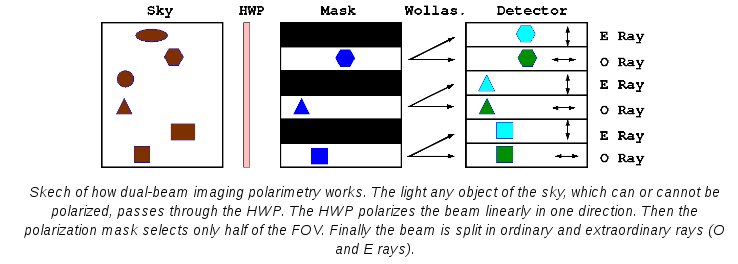
\includegraphics[scale=0.4]{img1.png}
\end{figure}
\end{itemize}

\end{frame}
\begin{frame}{Polarimetry}
\tdplotsetmaincoords{60}{120} 
\begin{tikzpicture} [scale=1.7, tdplot_main_coords, 
axis/.style={->, thick},
osc/.style={ blue, very thick   },
vector/.style={<->,red,very thick}]

%standard tikz coordinate definition using x, y, z coords

%tikz-3dplot coordinate definition using x, y, z coords


\node[tdplot_main_coords,anchor=south east] at (0,0,0){O};


\coordinate (x11) at (-0.5,0,0);
\coordinate (x12) at (0.5,0,0);
\coordinate (c1) at (0,1,0);
\coordinate (c2) at (0,3,0);


\coordinate (y2) at (2,0,0);

%\coordinate (O) at (0,2,0);


%draw axes
\draw[axis] (-1,0,0) -- (1,0,0) node[anchor=north east]{$\vec{e_2}$};
\draw[axis] (0,-1,0) -- (0,4,0) node[anchor=north west]{$y$};
\draw[axis] (0,0,-1) -- (0,0,1) node[anchor=south]{$\vec{e_1}$};

\draw[axis] (0,3,-1) -- (0,3,1) node[anchor=south]{$\vec{e_1}$};
\draw[axis] (0,1,-1) -- (0,1,1) node[anchor=south]{$\vec{e_1}$};


%draw a vector from O to P
 \begin{scope}[canvas is xz plane at y=1]
			\draw[osc] (c1) circle (0.5cm);
   \end{scope}
 \begin{scope}[canvas is xz plane at y=3]
			\draw[osc] (c2) circle (0.5cm);
   \end{scope}

\draw[red,very thick,->] (-0.51,3,-1.4) -- (0.51,3,1.4) node[anchor=south]{$\vec{e_1'}$};
\draw[red,very thick,->] (-1.4,3,0.51) -- (1.4,3,-0.51) node[anchor=south]{$\vec{e_2'}$};

\draw[red,very thick,->] (-0.75,1,-1.3) -- (0.75,1,1.3) node[anchor=south]{$\vec{e_f}$};
\draw[red,very thick,->] (-1.3,1,0.75) -- (1.3,1,-0.75) node[anchor=south]{$\vec{e_s}$};

\end{tikzpicture}
\begin{itemize}
\item $\vec{e_1}$, $\vec{e_2}$  reference system in object plane
\item $\alpha $ angle between $\vec{e_1}$ and $\vec{e_f}$ the fast axis of the retarder 
\item $\beta $ angle between $\vec{e_1}$ and $\vec{e_1'}$ one of the orthogonal axis of the wollaston prism: for example O-ray
\item $\delta$ phase difference between fast and slow axis induced by the retarder ($\pi$ in case of HWP)
\end{itemize}

\end{frame}

\begin{frame}{Polarimetry}
\begin{itemize}
\item at the entrance of the retarder in basis $\vec{e_1},\vec{e_2}$:
\begin{itemize}
\item $E_1 = \epsilon_1 e^{-i \omega t}$
\item $E_2 = \epsilon_2 e^{-i \omega t}$

\end{itemize}


\item rotation (in slow axis, fast axis basis: S.R of the retarder)
\begin{itemize}
\item $E_f = (\epsilon_1 cos \alpha + \epsilon_2 sin \alpha) e^{-i \omega t}$
\item $E_s = (-\epsilon_1 sin \alpha + \epsilon_2 cos \alpha) e^{-i \omega t}$
\end{itemize}
\item at the exit of the retarder (in the same basis: S.R of the retarder)
\begin{itemize}
\item $E_f = (\epsilon_1 cos \alpha + \epsilon_2 sin \alpha) e^{-i \omega t}$
\item $E_s = (-\epsilon_1 sin \alpha + \epsilon_2 cos \alpha)e^{i \delta} e^{-i \omega t}$
\end{itemize}
\item at the exit of the retarder (rotation $\beta - \alpha$ : in the S.R. of the wollaston prism)
the component along $\vec{e_1'}$:

$E_1' = cos(\beta - \alpha) E_f + sin(\beta - \alpha) E_s \implies $

$E_2' = -sin(\beta - \alpha) E_f + cos(\beta - \alpha) E_s \implies $


\begin{equation}
\begin{split}
E_1' = [cos(\beta - \alpha) (\epsilon_1 cos \alpha + \epsilon_2 sin \alpha) + \\
sin(\beta - \alpha ) (-\epsilon_1 sin \alpha + \epsilon_2 cos \alpha)e^{i \delta} ] 
e^{-i \omega t}
\end{split}
\end{equation}

\end{itemize}


\end{frame}

\begin{frame}{Polarimetry}

\begin{itemize}
\item $I \propto \epsilon_1 \epsilon_1^* + \epsilon_2 \epsilon_2^*$
\item $Q \propto \epsilon_1 \epsilon_1^* - \epsilon_2 \epsilon_2^*$
\item $U \propto \epsilon_1^* \epsilon_2 + \epsilon_1 \epsilon_2^*$
\item $V \propto i(\epsilon_1^* \epsilon_2 - \epsilon_1 \epsilon_2^*)$
\item signal O-ray (polarized along $\vec{e_1'}$) $ \propto <E_1' E_1'^*> \propto$  

$\frac{1}{2}[I + (Q cos 2\alpha + U sin 2 \alpha) cos(2(\beta - \alpha)) $

$- (Q sin 2\alpha - U cos 2 \alpha) sin(2(\beta - \alpha)) cos \delta $

$+ V  sin(2(\beta - \alpha)) sin \delta ]$

\end{itemize}

$\delta = 180^{\circ},\beta$ fixed $\implies$ in order to recover Stokes parameters we need 4 different values of $\alpha$:
the HWP rotates automatically(synchronized with the chopping and nodding) between the four position angles of 0$^{\circ}$, 45$^{\circ}$, 22.5$^{\circ}$ and 67.5$^{\circ}$
\end{frame}

\begin{frame}{Chop and nod}
To alleviate the effects of the bright background in mid-IR when performing imaging and low-resolution spectroscopy, 
a nearby position on the sky is observed frequently by moving the secondary mirror at a frequency of a few Hz 
(the telescope is said to chop between the target position and an adjacent sky position), 
and the pairs of images are subtracted. 
Moving the secondary mirror results in the telescope being seen by the detector in slightly 
different ways in the two secondary mirror positions. 
Since the telescope glows strongly at mid-IR wavelengths 
the subtraction leaves a residual radiative offset, 
which is much less than the telescope and sky brightnesses but is still significant. 
To get rid of (most of) this offset the entire telescope is moved or 
nodded typically about twice per minute. 
Normally the nod is set to be the same amplitude and direction as the chop, 
so that the science target switches chop positions between the two nod positions.

\end{frame}

\begin{frame}{Polarimetry}
\begin{figure}[H]
 \centering
 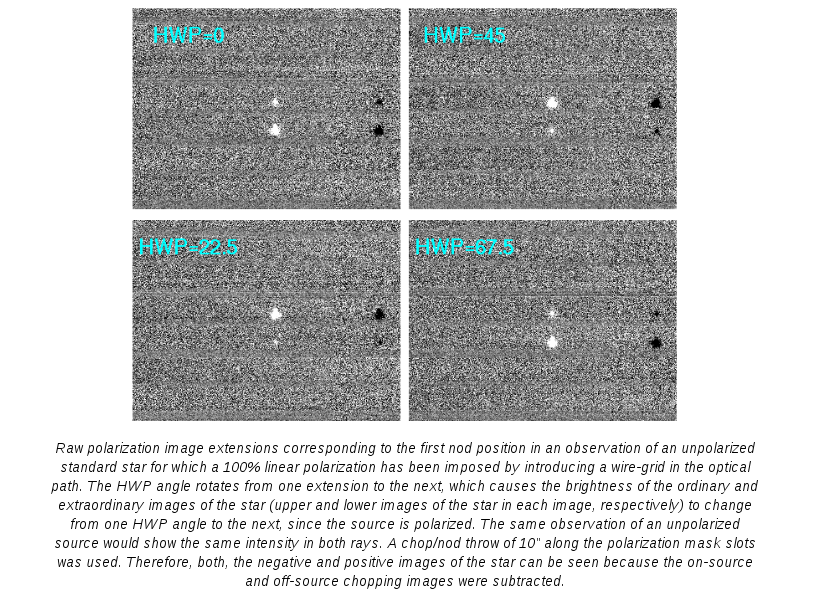
\includegraphics[scale=0.35]{img6.png}
\end{figure}
\end{frame}


\begin{frame}{Chop methods}
\begin{itemize}
\item The secondary mirror of the telescope is then moved slightly
away from the nominal position so that the program object moves out of the field of view
of the camera and another set of images is acquired. This procedure, called a “chop”
cycle, is repeated many times at typically a 2-10 Hz rate moving back and forth between 
"on-source" and "off-source" positions. A "chop-differenced" signal is formed by taking
the difference between the on-source and off-source images.

\item In the on-chip method, the
chopper throw is set to be less than the detector array field-of-view so that the source
remains "on chip" in both chopper positions, i.e. in both the "on-source" and "off-source"
chopper positions as referred to in the standard method. Note that since the source is present in both positions of the
chopper, the chop-differenced frame will contain both a positive and negative image of
the source 

\end{itemize}
\end{frame}


\begin{frame}{Polarimetry}



\begin{itemize}
\item dual beam polarimetry  in N band window with accuracy $> 99\%$ at the center wavelength $10.5 \mu m$
\item decreasing towards the cutoff wavelength of N window
\item $50\%$ field of view blocked by the mask (to avoid overlapping of orthogonally polarized beams emerging from the prism)
\item 2 beams $\implies$ high precision (the difference from standard polarimeter with 1 exit beam - along acceptance axis)
\end{itemize}
\end{frame}

\begin{frame}{Polarimetry}
\begin{itemize}
\item SNR needed in order to reach a certain polarization accuracy $\Delta P$ is given by:
\item $SNR = \frac{\sqrt{2}}{\Delta P}$
\item for example for a target with an expected polarization degree of $3\%$ we want a polarization accuracy of $1\%$ 
$\implies SNR = 141$
\item we use the SNR afterwards  when  calculating exposure time in the Canaricam Exposure Time Calculator
\begin{figure}[H]
 \centering
 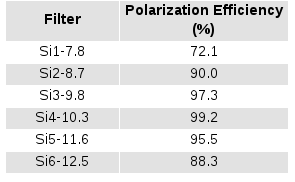
\includegraphics[scale=0.4]{img3.png}
\end{figure}
\end{itemize}
\end{frame}


\begin{frame}{Polarimetry}
\begin{itemize}
\item degree of instrumental polarization $0.6- 0.7\%$ across the N band window
\item reflection(which induces linear polarization) at the GTC flat tertirary mirror (M3) with a 45 degree angle of incidence, 
which is expected to produce most of the instrumental polarization
\item $\implies $ polarization angle (PA) in table above varies with changing the instrument position angle (IPA) and 
when the elevation of star evolves with time
\end{itemize}
\end{frame}


\begin{frame}{Polarimetry}
\begin{figure}[H]
 \centering
 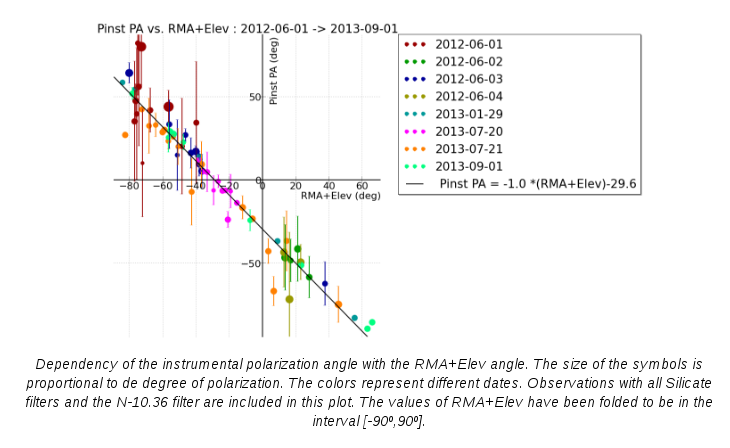
\includegraphics[scale=0.4]{img5.png}
\end{figure}
\end{frame}

\begin{frame}{Polarimetry}
\begin{figure}[H]
 \centering
 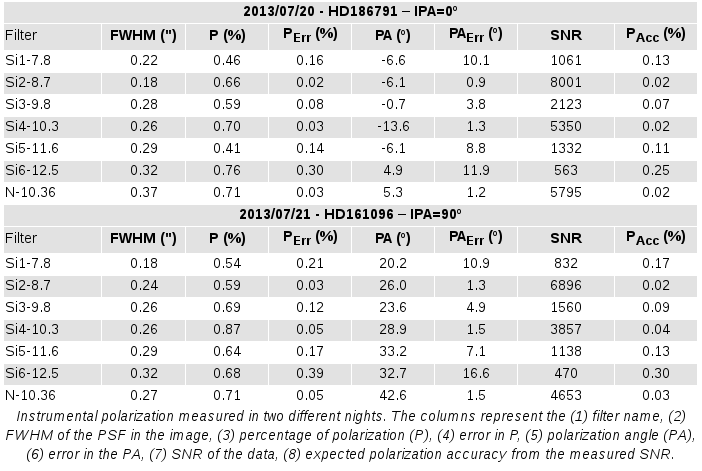
\includegraphics[scale=0.4]{img4.png}
\end{figure}
\end{frame}

\begin{frame}{Spectropolarimetry}
\begin{itemize}
\item the design permits having simultaneously the diffraction grating and the polarimeter
\item the 2 beams (linearly polarized in orthogonal directions) emerging from the polarizer (Wollaston prism) :  
are imaged on the detector as separate spectra because the diffraction grating is also in the optical path (afterwards)
\item as in polarimetry the field of view is reduced by $50\%$
\item The same formula as in the case of imaging polarimetry relates the SNR needed to reach a given polarization accuracy , 
but in this case the caculation must be done for each spectral resolution element
\item instrumental polarization consistent with imaging polarimetry results
\end{itemize}
\end{frame}

\begin{frame}{Spectropolarimetry}
Polarization Measurement Efficiency consistent with the efficiency table before (polarimetry)
\begin{figure}[H]
 \centering
 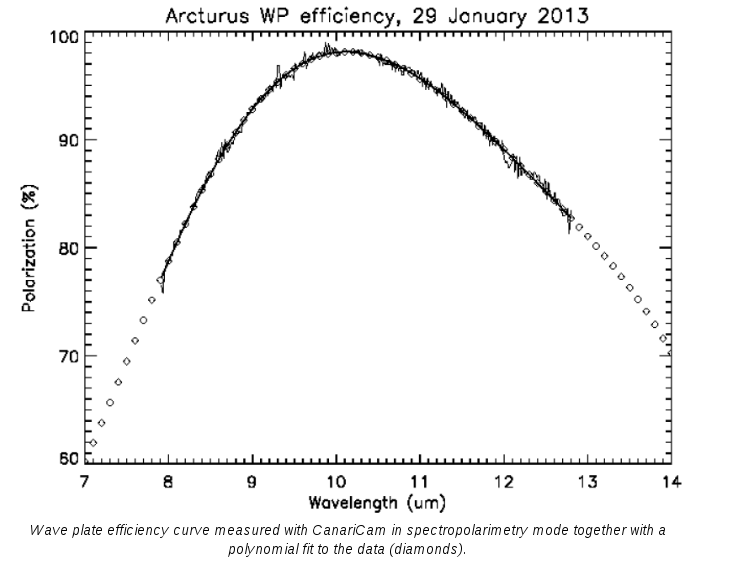
\includegraphics[scale=0.35]{img12.png}
\end{figure}
\end{frame}

\begin{frame}{Coronagraph}
\begin{itemize}
\item detect faint mid-IR point sources, such as
sub-stellar objects, and faint extended sources, such as circumstellar disks, that are
located very close to bright point sources and which might not be detectable without the
coronagraphic mode
\item occulting spot mask at the telescope focal plane:
sharp-edged (top hat), opaque metal disk with a
radius of 0.84 arcsec ($\frac{r}{f}$)

\item pupil mask at the first pupil plane inside camera: small central opaque disk for the
central obscuration supported by thin, slightly wedged, veins that mask the images of the secondary mirror
spider supports (and we need to keep them masked)  + large hexagonally shaped mask
that blocks the outer edges of the primary mirror 
\end{itemize}

\end{frame}
\begin{frame}{Coronagraph}
\begin{figure}[H]
 \centering
 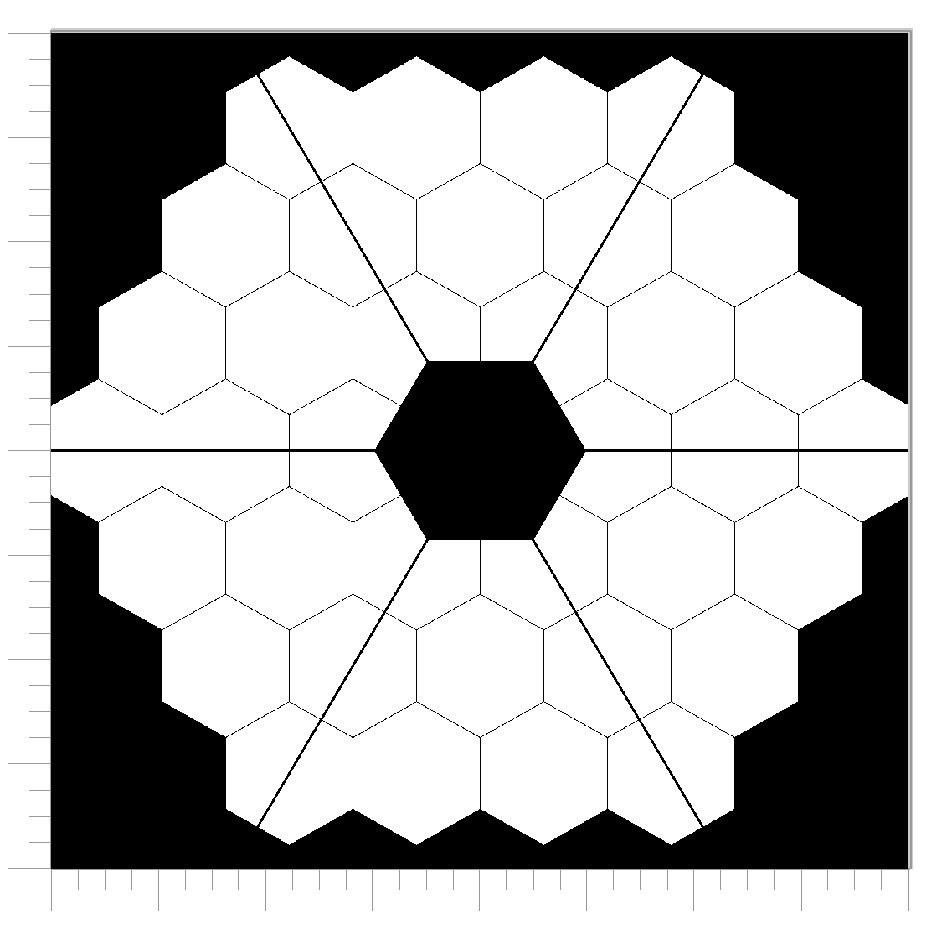
\includegraphics[scale=0.2]{Image82.jpg}
\caption{The shape of the GTC primary mirror}
\end{figure}

\end{frame}

\end{document}
